\documentclass[journal]{IEEEtran}
\usepackage[T1]{fontenc}
\usepackage{cite}
\usepackage{amsmath,amssymb,amsthm}
\newtheorem{proposition}{Proposition}
\usepackage{graphicx}
\usepackage{booktabs}
\usepackage{multirow}
\usepackage{array}
\usepackage{url}
\usepackage[hidelinks]{hyperref}
\graphicspath{{figures/}}

% ---- macros kept small and repeated verbatim (paper-voice rule 11) ----
\newcommand{\sys}{MCP}
\newcommand{\spraycheck}{SprayCheck}
\newcommand{\flowpulse}{FlowPulse}

\begin{document}

\title{What a Two-Byte Witness Buys on a Sprayed Fabric:\\ A Silicon-Measured Comparison of In-Fabric Grayhole Localization Against Passive Detection}

\author{Philip~Akekulip% <-this % stops a space
\thanks{P.~Akekulip is with [institution]. E-mail: akekulip@gmail.com.}%
\thanks{Manuscript received [date].}}

\markboth{IEEE/ACM Transactions on Networking}%
{Akekulip: What a Two-Byte Witness Buys on a Sprayed Fabric}

\maketitle

\begin{abstract}
Packet spraying spreads each flow of a machine-learning training job across every spine switch, so a link that silently drops a small fraction of its packets leaves its evidence divided among many paths. A detector that only counts arrivals then faces two limits: the deficit it looks for shrinks with the loss rate while the sampling noise of spraying does not, and an arrival deficit at a leaf is the product of an uplink and a downlink survival rate, so one vantage cannot tell the two directed links apart. The two most recent passive detectors for sprayed fabrics accept both limits. In this paper, we measure what an in-fabric per-directed-link witness buys against them. The witness is an existing primitive: two bytes per packet and two counters per directed link. We replay both passive detectors over one shared stream of sprayed traffic and measure the ledger on an Intel Tofino switch. The witness detects at a flat cost of about twenty-two million packets from a loss rate of 1.5 percent down to one in ten thousand, where the passive cost grows past one hundred million packets and then past the budget. It names the exact directed link where the passive detectors return the uplink and downlink pair, it recovers injected loss exactly on silicon with no false positive, and it costs about 0.14 percent of a 1400-byte payload. The advantage holds for several independent faults and fails under a fleet-wide shift in loss, where a relative passive test is better.

\end{abstract}

\begin{IEEEkeywords}
Data center networks, packet spraying, gray failure, network telemetry, programmable switches.
\end{IEEEkeywords}

\section{Introduction}
\label{sec:intro}

Training fabrics for large machine-learning models spray packets. Instead of pinning a flow to one path, the leaf switch sends consecutive packets of the same flow to different spines, which balances load across a Clos fabric and is now the default of the Ultra Ethernet transport~\cite{spraying,uec,reps}. Spraying also changes what a failure looks like. A link that drops one packet in a thousand, or one in ten thousand, does not take a flow down. It slows every flow a little, because every flow crosses it. Such gray failures are common in production fabrics and hard to attribute~\cite{grayfailure,corropt}, and they can be costly for synchronous training jobs whose collective operations wait for the slowest packet~\cite{aegis}. We call a link that silently drops a small fraction of its packets a grayhole, and we call the problem of naming the directed link that carries it grayhole localization.

Grayhole localization on a sprayed fabric is challenging, due to two reasons. First, the evidence is divided. A flow that used to concentrate its loss on one path now spreads it across $k$ spines. Consequently, the per-path deficit a passive observer can see is $1/k$ of the fault, and it shrinks further as the loss rate falls, while the sampling noise of spraying, i.e., the variation in how many packets each spine happens to receive, does not shrink at all. Second, the evidence is aliased. A packet from one leaf to another crosses two directed links, an uplink into a spine and a downlink out of it. An arrival counter at the destination sees only the product of the two survival rates, and thus, a single vantage that counts arrivals can name a spine but cannot, by itself, tell the uplink from the downlink.

The two most recent detectors built for sprayed fabrics accept both limits. SprayCheck~\cite{spraycheck} applies a Z-test to per-spine arrival counts and resolves a directed link by intersecting reports from several leaves. FlowPulse~\cite{flowpulse} compares each ingress port's load against a learned baseline and applies a per-sender rule. Both are passive: they add nothing to the wire, they run on counters the switch already has, and they can be deployed today. However, a test on arrival counts needs enough packets for a deficit of fraction $p$ to stand above spray noise, and that number grows at least as $1/p$. Both papers also state that one report can only flag the uplink and downlink pair~\cite{spraycheck,flowpulse}.

An in-fabric witness can remove both limits by construction. The sending leaf stamps every packet with a per-directed-link sequence number. The receiving switch keeps, per directed link, the highest sequence number seen and the number of packets seen. The difference of the two deltas is then the loss on that directed link and nothing else. This primitive is not new. NetSeer~\cite{netseer}, LinkGuardian~\cite{linkguardian}, LossRadar~\cite{lossradar}, and the link-layer retry of Ultra Ethernet~\cite{uec} all place a per-link sequence witness in the data plane. What none of them reports is what the witness buys, and costs, on a sprayed fabric at the loss rates where the passive state of the art fails. That measurement, head-to-head against the passive detectors and on real silicon, is the contribution of this paper. We implement the witness as a receiver ledger on an Intel Tofino switch~\cite{tofino}, with a two-byte stamp and two registers per directed link, and we treat it as the measured arm of a comparison rather than as a new design.

To make the comparison fair, we replay SprayCheck and FlowPulse from their own papers, with their own thresholds and their own localization rules. All three detectors read one shared stream of sprayed traffic, and each sees it only through the counters its own switch would have. We run fifty seeds per loss rate from 1.5 percent down to $10^{-4}$, and we report false positives next to every action rate. Where a passive detector ties or beats the witness, we report it as plainly as where it does not. Our contributions are as follows.

\begin{itemize}
\item \textbf{Measures the detection cost-scaling separation.} The witness detects a single-link grayhole on the first epoch after onset at every loss rate. Its median cost is a flat 22.0 million fleet packets from 1.5 percent to $10^{-4}$, with an action rate of 1.00 and no false positive. SprayCheck's median cost grows from 24 million to 114 million packets as the loss rate falls to $10^{-3}$, its action rate falls from 1.00 to 0.78, and at $10^{-4}$ it detects nothing within the same 160-million-packet budget. FlowPulse fails one order of magnitude earlier. We show that this is a scaling law of any arrival-count test and not an artifact of the budget (Section~\ref{sec:detection}).
\item \textbf{Measures directed-link localization under spraying.} The witness names the exact directed link, and only it, at every loss rate and for both uplink and downlink faults. SprayCheck ties it at 1.0 to 1.5 percent loss, which we report as a null result, and degrades to the ambiguous uplink and downlink pair at $10^{-3}$. FlowPulse cannot detect an uplink fault at any rate once several senders share the port (Section~\ref{sec:localization}).
\item \textbf{Measures the ledger on silicon.} On a Tofino switch the ledger recovers injected loss exactly from $10^{-2}$ down to $10^{-4}$, i.e., six drops in sixty thousand packets, with zero false positives on more than forty thousand clean packets. The result holds for scheduled drops and for random per-packet drops, and a downlink grayhole is attributed to the downlink alone with zero false attribution on seven active sublinks (Section~\ref{sec:silicon}).
\item \textbf{Bounds the claim with a correlated-fault gate.} Under two or three simultaneous independent faults the witness's advantage widens, because the passive intersection produces spurious links. Under a fleet-wide shift in loss with no single culprit the witness fails and flags all 64 directed links, and SprayCheck's relative test is the better tool. We report both, and we scope every other claim to independent per-directed-link faults (Section~\ref{sec:robustness}).
\item \textbf{Quantifies the cost.} The two-byte witness adds about 0.14 percent to a 1400-byte payload and six bytes of register state per directed link. It also costs one ingress pipeline stage, which brings the program to the twelve-stage ceiling of the Tofino~1 (Section~\ref{sec:cost}).
\end{itemize}

To the best of our knowledge, this is the first head-to-head measurement of an in-fabric per-directed-link witness against the passive sprayed-fabric detectors, on the loss regime all three target, and on silicon. We claim no novelty for the witness itself. The per-link sequence stamp is the primitive of NetSeer and LinkGuardian, and the localization advantage we measure is a property of the information the witness holds rather than of a better inference. What the paper adds is the measurement, its cost, and its boundary.

The rest of the paper is organized as follows. Section~\ref{sec:background} describes sprayed fabrics, grayholes, the fault model, and the objectives we evaluate. Section~\ref{sec:ledger} describes the receiver ledger as implemented. Section~\ref{sec:method} describes the replay harness, the two passive baselines, and the silicon testbed. Sections~\ref{sec:detection} to~\ref{sec:cost} report detection cost, localization, the silicon measurements, the correlated-fault gate, and the cost. Section~\ref{sec:discussion} discusses limitations, Section~\ref{sec:related} positions the work against prior systems, and Section~\ref{sec:conclusion} concludes.

\section{Background, Fault Model, and Objectives}
\label{sec:background}

\subsection{Sprayed Leaf--Spine Fabrics}

A two-tier Clos fabric connects $n$ leaf switches to $k$ spine switches, and every leaf has one link to every spine. A packet from leaf $L_a$ to leaf $L_b$ crosses exactly two directed links: the uplink $L_a\!\rightarrow\!S_i$ and the downlink $S_i\!\rightarrow\!L_b$ for some spine $S_i$. We call each such one-way hop a \emph{directed link}. A fabric with $n$ leaves and $k$ spines has $2nk$ of them. Under per-packet spraying the leaf chooses the spine for each packet independently, in the simplest case uniformly at random~\cite{spraying}. A flow of $N$ packets then places about $N/k$ packets on each of its $k$ uplinks and on each of its $k$ downlinks. The Ultra Ethernet specification adopts spraying as its default and adds a link-layer retry that can retransmit a lost frame across one link~\cite{uec}. REPS extends spraying with a load balancer that steers away from paths that show loss~\cite{reps}. Throughout the paper we use $n=4$ and $k=8$ in the replay harness, which is the topology SprayCheck evaluates~\cite{spraycheck}, and a 4-leaf, 2-spine virtual fabric on silicon.

A \emph{grayhole} is a directed link that forwards most of its packets and silently drops a fraction $p$ of them. We study $p$ from 1.5 percent down to $10^{-4}$, and we call $10^{-3}$ to $10^{-4}$ the low-loss regime. A grayhole differs from a blackhole, which drops everything and is caught by any liveness check. It also differs from congestion loss, which is transient and is shared by every link behind the congested queue. Time is divided into \emph{epochs}, i.e., the period at which a controller reads counters and decides. In the replay harness one epoch carries two million packets across the fleet, and the detectors act at epoch boundaries.

\subsection{Two Limits of a Passive Vantage}
\label{sec:limits}

A passive detector counts packets the switch already forwards and adds nothing to them. Under spraying it faces two limits, and both become worse as $p$ falls.

\textbf{The cost limit.} A grayhole of rate $p$ on one of $k$ spines removes a fraction $p$ of the packets that spine should have received. To notice the deficit, a passive detector compares that spine's arrival count against the others, and the comparison is only meaningful when the expected deficit exceeds the sampling noise of spraying. A witness that observes each directed link's own transmit count compares the link's loss count against the background loss floor $f$ instead. Both comparisons are Poisson separations, and both scale the same way in $p$; what differs is the constant. We state this as a proposition, because it governs every detection number in the paper.

\begin{proposition}[Detection cost of a count test and of a witness]
\label{prop:cost}
Let a directed link carry $\lambda$ packets per epoch, let spray decisions and per-packet drops be independent, and let a test require $s$ standard deviations of separation. A passive test on arrival counts separates a loss fraction $p$ from spray noise, which has standard deviation $\sqrt{\lambda}$, when $\lambda p > s\sqrt{\lambda}$, i.e., when
\begin{equation}
\lambda_{\mathrm{passive}} > s^2 / p^2 .
\label{eq:passive}
\end{equation}
A witness that counts the link's own drops separates them from a background floor $f<p$, whose drops have standard deviation $\sqrt{\lambda f}$, when $\lambda p > s\sqrt{\lambda f}$, i.e., when
\begin{equation}
\lambda_{\mathrm{witness}} > s^2 f / p^2 .
\label{eq:witness}
\end{equation}
\end{proposition}
\noindent The two bounds have the same $1/p^2$ form; the witness divides the constant by $f$, which is $10^5$ on a fabric whose floor is $10^{-5}$. The Gaussian form of~\eqref{eq:witness} holds when the floor produces many drops per epoch; when $\lambda f$ is below about one, the separation is a sparse Poisson test and the required $\lambda$ grows as $1/(p\log(p/f))$ instead, which is milder in $p$ but diverges as $p$ approaches $f$. Two consequences follow, and Section~\ref{sec:detection} measures both. First, over any range of $p$ for which one epoch's $\lambda$ already exceeds $s^2 f/p^2$, the witness detects on the first epoch and its cost looks flat; that is a statement about the epoch volume relative to the floor, not about the absence of a wall. Second, the witness has a wall of its own, at $p$ of a few times $f$, and the wall moves with $f$.

\textbf{The aliasing limit.} An arrival counter at $L_b$ for packets that came through spine $S_i$ sees the product of the survival rates of $L_a\!\rightarrow\!S_i$ and $S_i\!\rightarrow\!L_b$. One counter alone cannot tell which of the two directed links dropped the packets. SprayCheck resolves the pair by intersecting failure reports from several leaves that share the spine~\cite{spraycheck}. FlowPulse resolves it by asking whether every sender on the port is affected or only one~\cite{flowpulse}. Both rules need corroborating traffic, and that traffic can become scarce at low loss. A per-directed-link witness holds each link's own count and needs no corroboration. Section~\ref{sec:localization} measures both.

\subsection{Fault Model, Objectives, and Scope}
\label{sec:scope}

We assume that the loss rate of a faulty directed link is stationary over the observation window and that faults on different directed links are independent. We argue that this is a reasonable assumption for the physical-layer causes that dominate gray failures in production, i.e., damaged optics, marginal cables, and misconfigured forward error correction. Each of these is local to one link and persists until repaired~\cite{corropt}. We assume that a healthy directed link has a small background loss rate, set to $10^{-5}$ in the harness, and we assume that one or several directed links can be faulty at once. We also assume that congestion loss is negligible on the measurement timescale, as on a lossless fabric with priority flow control or one provisioned so that queue drops are rare; this is a precondition of the absolute-floor test rather than a convenience, because the test counts a queue's drops exactly as it counts a link's, and Section~\ref{sec:robustness} shows what happens when the assumption fails. We do not assume that the faulty link is known to carry any particular flow, and we do not assume that the controller can inject probes.

The paper evaluates four objectives, and we refer to them by label in the rest of the paper.
\begin{itemize}
\item \textbf{O1, detection cost.} The number of packets, and the fraction of trials, a detector needs to flag the faulty spine or link within a fixed budget, as a function of $p$, with the false-positive rate reported next to it.
\item \textbf{O2, localization.} Whether the detector names exactly the faulty directed link, an ambiguous set that contains it, or nothing.
\item \textbf{O3, silicon fidelity.} Whether the ledger, on a real switch, recovers the injected loss exactly at each $p$ and attributes it to the injected directed link alone.
\item \textbf{O4, the boundary.} Whether O1 and O2 survive several simultaneous faults, and whether they survive a fleet-wide, correlated shift in loss.
\end{itemize}

\textbf{Scope.} Two regimes are out of scope for the headline claims. Under a common-mode shift, in which every link's loss rises together, the ledger's decision rule fails, as Section~\ref{sec:robustness} shows and Section~\ref{sec:discussion} discusses. The claims of Sections~\ref{sec:detection} to~\ref{sec:silicon} are therefore stated for independent faults on a stationary fabric. Repairing or re-admitting a faulty link is not addressed; Section~\ref{sec:related} cites the systems that do. Blackholes are used only to validate the testbed and are not part of the evaluation.

\section{The Receiver Ledger}
\label{sec:ledger}

The receiver ledger is the measured arm of this paper. It is our implementation of the per-link sequence witness that NetSeer~\cite{netseer} and LinkGuardian~\cite{linkguardian} place in the data plane, at reduced width, and we describe it here only far enough that the cost and the measurements of the later sections can be read. We claim no design contribution for it. In Figure~\ref{fig:system}, we show the data path from a sending leaf to a receiving leaf and the two places the ledger touches it.

\begin{figure}[t]
\centering
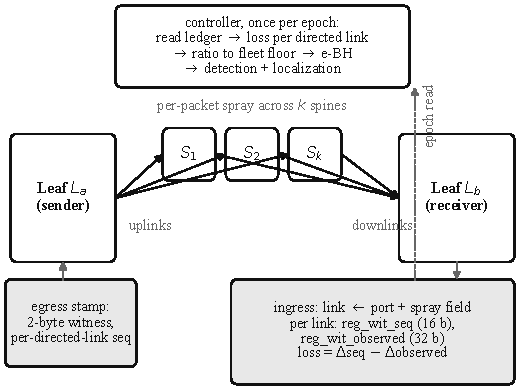
\includegraphics[width=\columnwidth]{fig_system.pdf}
\caption{The receiver ledger on a sprayed leaf--spine fabric. The sending leaf stamps each packet at egress with a two-byte per-directed-link sequence number. The receiving switch reconstructs the directed link from its own ingress port and the spray field, and keeps two registers per directed link: the last sequence number seen and the number of packets seen. Once per epoch the controller reads both registers, takes the difference of their deltas as the loss on that directed link, compares it with the fleet floor, and applies e-BH to name the faulty links.}
\label{fig:system}
\end{figure}

\textbf{Witness stamp.} At the egress of the sending hop, the switch inserts a two-byte header carrying a 16-bit sequence number that it increments per directed sublink, i.e., per directed link and traffic class. The header carries nothing else. An earlier version of the ledger also carried a 16-bit link identifier, which doubled the wire cost. Because the receiving hop already knows its own ingress port, and because the spray field is already on the wire for load balancing, the identifier is redundant, and we removed it. Section~\ref{sec:cost} reports what that removal cost in pipeline stages. The stamp is an in-fabric cost only: it is stripped before the packet reaches a host.

\textbf{Link reconstruction.} At the ingress of the receiving hop, a match table keyed on the ingress port and the spray field names the directed link, and a second table appends the traffic class, which the switch classifies fresh for every packet from the packet's size and its differentiated-services code point. Two tables are needed rather than one because the traffic class is a per-packet property, not a per-link one; a single table that baked a fixed class into each link entry would mislabel every packet whose class differed from the entry.

\textbf{Ledger registers.} For each of the $2nk$ directed links, and for each traffic class, the receiving switch keeps two registers: $\mathit{seq}$, the 16-bit sequence number of the last stamped packet seen on that sublink, and $\mathit{obs}$, a 32-bit lifetime count of the stamped packets seen. Both can be updated in the data plane at line rate, and both were on our switch. Over an epoch in which the two registers advance by $\Delta\mathit{seq}$, taken modulo $2^{16}$, and $\Delta\mathit{obs}$, the loss on the sublink is
\begin{equation}
\ell = \Delta\mathit{seq} - \Delta\mathit{obs},
\label{eq:loss}
\end{equation}
because the sender advanced the sequence once per packet it sent and the receiver counted once per packet that arrived. Equation~\eqref{eq:loss} is exact for in-order and for reordered arrivals. Because the sequence register keeps a frontier rather than a running sum, a late packet manufactures no phantom loss. A duplicated packet drives the estimate to $-1$, which the controller can read as a duplicate. A packet lost after the last survivor of an epoch is counted in the next epoch, when the next survivor advances the frontier. We verified all three properties against the compiled program on the vendor's software model before any hardware measurement (Section~\ref{sec:method}).

\textbf{Decision.} Once per epoch the controller reads every sublink's registers, forms the loss ratio $\ell/\Delta\mathit{seq}$, and compares it with the fleet floor, a leave-one-out estimate of the background loss rate that excludes the sublink under test. Because a healthy sublink's ratio sits at the floor while a faulty one sits far above it, the controller can test each sublink on its own evidence. It never compares a sublink against the sampling noise of the other spines. The per-sublink evidence is accumulated as an e-process. The set of sublinks whose evidence exceeds the e-BH threshold at a chosen false discovery rate~\cite{ebh} is the set the controller names as faulty. That set is both the detection and the localization, because a rejected sublink is a directed link and only the link that lost packets can have an anomalous ratio. We note that this decision rule is the part of the ledger that fails under a fleet-wide shift in loss, because the floor then moves with the fault (Section~\ref{sec:robustness}).

\section{Methodology}
\label{sec:method}

The evaluation has two vehicles. A replay harness compares the ledger with the two passive detectors on one shared stream of sprayed traffic, because the passive detectors are host-side systems that cannot run on our fabric and because a head-to-head needs every arm to see the same packets. A silicon testbed then measures the ledger's own side of that comparison on a real switch. In this section, we describe the harness, the three arms, the metrics, and the testbed.

\subsection{The Replay Harness}

\textbf{Shared stream.} Every epoch, the harness draws one per-packet spray decision and one per-hop survival outcome for every packet, and it feeds the same draw to all three arms. Spray is independent and uniform across the $k=8$ spines, which matches SprayCheck's own model and FlowPulse's temporal-symmetry assumption~\cite{spraycheck,flowpulse}. Survival is independent per directed link with rate $1-p$ on a faulty link and $1-10^{-5}$ on a healthy one. Each arm sees only what its own switch would see. The ledger arm receives the exact per-sublink transmit and receive counts its registers produce. The SprayCheck arm receives receive-only per-spine arrival counts; no transmit count and no drop count exists in its interface, so none can be passed to it by mistake. The FlowPulse arm receives receive-only per-port load, predicted from its own bootstrapped history, and never the ledger's transmit ground truth.

\textbf{Scenario.} Each trial runs ten epochs of clean traffic, during which FlowPulse bootstraps its baseline and the ledger warms its floor. The trial then degrades one spine, or one directed link, to the target rate $p$ for the rest of the run. For detection (O1) the fleet carries two million packets per epoch, and a trial ends when the arm flags the faulty spine or after 80 post-onset epochs, a budget of 160 million packets. For localization (O2) the harness extends to the two-hop fabric of $n=4$ leaves, and each ordered leaf pair carries two million packets per epoch. The localization budget is 60 post-onset epochs, which is deliberately generous to the passive arms so that SprayCheck can complete a corroborating round of measured flows. For the correlated gate (O4) the window is 40 post-onset epochs. We run 50 seeds per cell.

\textbf{Two fidelity checks that changed the harness.} Before trusting any number we checked each arm against its own paper. Two checks failed and were fixed. First, a per-packet traffic generator made one two-million-packet epoch take tens of seconds; we vectorized it with a multinomial draw, which changed no distribution. Second, at an initial volume of 200 thousand packets per epoch, FlowPulse's fixed one-percent threshold false-alarmed on a healthy spine in every trial. The reason is that the relative spray noise at that volume, about 0.6 percent, sat close to its threshold. We raised the volume to two million packets per epoch, at which its false-positive rate on healthy spines is 0.0000, consistent with the paper's own claim of under one percent~\cite{flowpulse}. We report that rate next to every result.

\subsection{The Three Arms}

\textbf{The ledger.} The controller of Section~\ref{sec:ledger}, unmodified from the version measured on silicon, runs over the exact per-sublink counts. Its localized set is the set of sublinks e-BH rejects.

\textbf{SprayCheck-Z.} We reimplement SprayCheck's detector from its paper~\cite{spraycheck}: a Z-test on per-spine arrival counts with sensitivity $s$ calibrated under the paper's own Poisson model at 2.5 million packets per spine, which gives $s=3.24$. For localization we implement its full cross-leaf rule: a report flags the uplink and downlink pair of a path, and a single link is named only when it lies in the intersection of reports from different leaves. SprayCheck's real spraying uses join-the-shortest-of-two-queues, which has less noise than the Poisson model; a sensitivity tuned to that would shift its cost curve down by a constant factor but not change how the cost scales with $p$.

\textbf{FlowPulse-$\theta$.} We reimplement FlowPulse's port-load detector with its fixed one-percent threshold against a learned per-port baseline, and its per-sender localization rule: if every sender on an ingress port is affected the local downlink is named, and if only one sender is affected the uplink from that sender's leaf is named~\cite{flowpulse}. We give the arm per-sender visibility on every port, which its paper assumes; this is the charitable reading, not a weakened one.

\subsection{Metrics}

\textbf{Action rate} is the fraction of the 50 seeds in which the arm flags the faulty spine or link within the budget, with a 95 percent Wilson interval~\cite{wilson}. \textbf{Packets to detect} is the fleet-wide packet count from the fault's onset to the first correct flag, reported as a median with its interquartile range over the seeds that detected; we mark it as survivorship-biased wherever the action rate is below one. \textbf{False positive} is any healthy spine or link flagged, reported next to every action rate. For O2, \textbf{exact} means the arm named the true directed link and only it, \textbf{ambiguous} means it named a set that contains a healthy link, and \textbf{miss} means it named nothing. We also report the mean set size over detections and a paired exact McNemar test between arms on the same seeds. For O4, \textbf{recall} is the fraction of true faulty links named, and \textbf{exact-all} is the fraction of seeds that named the true set and nothing else. We report the false-positive rate both over the whole window and at its final epoch, so that a transient false flag can be separated from a persistent one.

\subsection{The Silicon Testbed}

\textbf{Switch.} The ledger runs on an Intel Tofino~1 switch~\cite{tofino} with SDE 9.13.2. A 4-leaf, 2-spine virtual fabric is emulated on the switch itself: a four-lane 25~Gb/s direct-attach cable loops four front-panel ports back to the switch, and each directed virtual link is one traffic-manager queue on one loop port. With four traffic classes, the program tracks 1024 sublinks. The pipeline occupies 12 ingress and 5 egress match-action stages (Section~\ref{sec:cost}).

\textbf{Traffic and ground truth.} A server with a 25~Gb/s network interface sends 1400-byte packets at 20 thousand packets per second, and a differentiated-services code point selects the traffic class and thus the sublink. Two fault injectors run in the switch's egress pipeline. The exact injector drops exactly $D$ stamped packets on a chosen sublink, so the ground truth is $D$. The stochastic injector draws a 16-bit random value per packet and drops the packet when the value falls below $W=\lfloor p\cdot 2^{16}\rceil$, so it drops each packet with probability $W/2^{16}$. For this injector the ground truth is its own direct counter of packets dropped, read from the switch, because a random injector has no preset count. Every cell reads a baseline census immediately before arming and reports deltas against it. Every cell also keeps $\Delta\mathit{seq}$ below $2^{16}$, so that the sequence wraps at most once, and clears both injectors before and after. The recovered loss is Equation~\eqref{eq:loss} read through the controller's census.

\textbf{Model validation.} Before any hardware run, the compiled program passed nine correctness tests on the vendor's software model. They cover the exact recovery of injected loss, the invisibility of a trailing loss until the next survivor, the 32-bit transmit frontier past 255 and 256 packets, the absence of phantom loss under reordering, the $-1$ signature of a duplicate, and the realized rate of the stochastic injector, which fell within four standard deviations of its target. The hardware measurements of Section~\ref{sec:silicon} were then taken on the same build.

\section{Detection Cost (O1)}
\label{sec:detection}

Proposition~\ref{prop:cost} predicts three things: the passive cost grows as $1/p^2$; the witness's cost is set by the epoch volume until $p$ approaches the floor $f$, where it has a wall of its own; and a zero-byte counter pair with the same information as the witness is separated from it only by read skew. This section measures all three. Packets to detect are counted from the fault's onset. In Figure~\ref{fig:scaling} and Table~\ref{tab:detection}, we show the packets each arm needed to flag the faulty spine and the fraction of seeds in which it did so, for eight loss rates from 1.5 percent down to the floor of $10^{-5}$.

\begin{figure}[t]
\centering

\includegraphics[width=\columnwidth]{scaling_curve.pdf}
\caption{Median post-onset packets to detect a single-spine grayhole against loss rate $p$, over 50 seeds, $k=8$ spines, and a budget of 80 post-onset epochs of 2 million packets (dotted ceiling); shaded bands are interquartile ranges. Filled markers are cells with an action rate of 1.00; hollow markers are annotated with the fraction of seeds that detected, and their median is over those seeds only; a cross on the ceiling marks a cell in which no seed detected. The ledger's cost is one epoch until the loss rate nears the floor, then rises to its own wall; the passive detectors' cost grows toward the ceiling and crosses it two decades earlier.}
\label{fig:scaling}
\end{figure}

\begin{table}[t]
\caption{Detection of a single-spine grayhole within a budget of 80 post-onset epochs (160 million packets), 50 seeds per cell: action rate (Act.) and, over the seeds that detected, the median post-onset packets to the first correct flag (Pkts). The 95 percent Wilson interval is [0.93, 1.00] for every 1.00, [0.65, 0.87] for 0.78, [0.26, 0.52] for 0.38, and [0.00, 0.07] for every 0.00. False positives were 0.00 for every arm at every rate.}
\label{tab:detection}
\centering
\footnotesize
\begin{tabular}{@{}lcccccc@{}}
\toprule
 & \multicolumn{2}{c}{Ledger} & \multicolumn{2}{c}{SprayCheck-Z} & \multicolumn{2}{c@{}}{FlowPulse-$\theta$} \\
\cmidrule(lr){2-3}\cmidrule(lr){4-5}\cmidrule(l){6-7}
$p$ & Act. & Pkts & Act. & Pkts & Act. & Pkts \\
\midrule
1.5\%     & 1.00 & 2\,M & 1.00 & 4\,M & 1.00 & 2\,M \\
1.0\%     & 1.00 & 2\,M & 1.00 & 6\,M & 1.00 & 2\,M \\
0.5\%     & 1.00 & 2\,M & 1.00 & 12\,M & 0.38 & 68\,M \\
$10^{-3}$ & 1.00 & 2\,M & 0.78 & 94\,M & 0.00 & -- \\
$10^{-4}$ & 1.00 & 2\,M & 0.00 & -- & 0.00 & -- \\
$5\!\times\!10^{-5}$ & 1.00 & 6\,M & 0.00 & -- & 0.00 & -- \\
$2\!\times\!10^{-5}$ & 1.00 & 36\,M & 0.00 & -- & 0.00 & -- \\
$10^{-5}$ ($=f$) & 0.00 & -- & 0.00 & -- & 0.00 & -- \\
\bottomrule
\end{tabular}
\end{table}

\textbf{The ledger detects on one epoch until the floor is near.} From 1.5 percent down to $10^{-4}$ the ledger flagged the faulty spine in every seed on the first epoch after onset, at a cost of 2 million fleet packets with an interquartile range of 2 to 2 million, widening to 2 to 4 million at $10^{-4}$. The reason is that one epoch carries 250 thousand packets per spine, which exceeds the $s^2 f/p^2$ of Proposition~\ref{prop:cost} at every rate in that range, so the first epoch's drops can already stand above the floor. Below $10^{-4}$ the wall appears where the proposition puts it. At $5\times10^{-5}$ the median cost rose to 6 million packets and at $2\times10^{-5}$ to 36 million, still with an action rate of 1.00 and no false positive. At the floor itself, $10^{-5}$, no seed detected, because a link that loses at the background rate is not a fault by the ledger's own definition. The flat portion of the curve is therefore a statement about the epoch volume relative to the floor, and the paper no longer calls it flat without that qualification.

\textbf{The passive cost grows as $1/p^2$ and the action rate collapses.} SprayCheck-Z needed 4, 6, and 12 million packets at 1.5, 1.0, and 0.5 percent, i.e., two, three, and six epochs. At $10^{-3}$ its median rose to 94 million packets, 47 times the ledger's, and that median is over the 78 percent of seeds that detected at all; its interquartile range widened from 4 to 4 million at 1.5 percent to 62 to 128 million at $10^{-3}$. At $10^{-4}$ and below no seed detected within the budget. FlowPulse-$\theta$ failed one order of magnitude earlier: it matched the ledger at 1.5 and 1.0 percent, detected in 38 percent of seeds at 0.5 percent with a median of 68 million packets, and detected nothing at $10^{-3}$ and below. Both passive arms had a false-positive rate of 0.00 at every rate, so the collapse is a loss of sensitivity, not a trade against false alarms. The separation is visible inside the budget: the 22 percent SprayCheck missed at $10^{-3}$ and its whole column at $10^{-4}$ are the same $s^2/p^2$ wall pushed past 160 million packets. A larger budget would move the passive floor to a rarer $p$ but cannot change the exponent; the ledger's curve would not move at all, because within its flat range it detects on the first epoch. This is a statement about cost, not capability: a passive detector with an unbounded budget can eventually detect at $10^{-4}$, and nothing here says otherwise.

\begin{figure}[t]
\centering
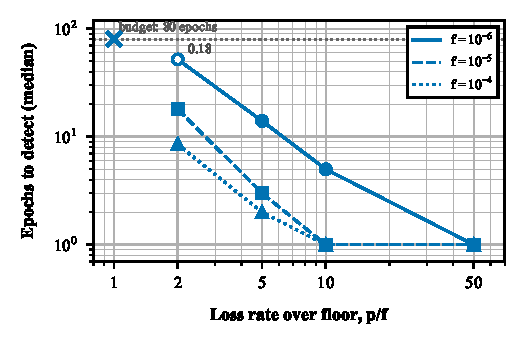
\includegraphics[width=\columnwidth]{fig_floor.pdf}
\caption{The ledger's wall tracks the floor: median epochs to detect against the loss rate as a multiple of the background floor $f$, for three floors, 50 seeds per cell. A cross at the top marks a cell in which no seed detected within 80 epochs; a hollow marker is annotated with its action rate. At every floor the ledger detects nothing at $p=f$, detects in every seed from about $5f$ upward, and reaches one epoch by $10f$ to $50f$.}
\label{fig:floor}
\end{figure}

\textbf{The wall moves with the floor.} Figure~\ref{fig:floor} repeats the ledger arm at three background floors, $10^{-6}$, $10^{-5}$, and $10^{-4}$, over $p$ from $f$ to $50f$. The curves align when plotted against $p/f$. At $p=f$ nothing is detected at any floor. At $2f$ the action rate is 1.00 at the two higher floors, in a median of 18 and 8.5 epochs after onset, and 0.18 at $10^{-6}$, where the floor produces half a drop per epoch and the separation is the sparse Poisson case of the proposition. From $5f$ upward every seed detects, in a median of 14, 3, and 2 epochs after onset at floors of $10^{-6}$, $10^{-5}$, and $10^{-4}$, falling to one epoch by $50f$, $10f$, and $10f$. Consequently, we expect the loss rate at which the witness stops paying to be not a fixed number but a small multiple of whatever the fabric's background floor is, which production floors can put anywhere from $10^{-6}$ to $10^{-4}$~\cite{corropt}. SprayCheck's action rate at a fixed $p$ barely changes with the floor, since its noise is spray noise rather than floor noise: 0.16 at $p=5\times10^{-4}$ over a $10^{-5}$ floor and 0.06 over $10^{-4}$.

\begin{figure*}[t]
\centering
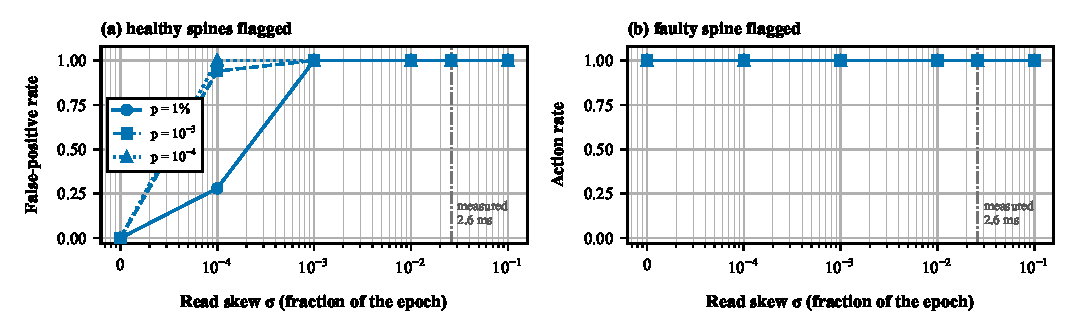
\includegraphics[width=\textwidth]{fig_counterpair.pdf}
\caption{The zero-byte counter pair against controller read skew, 50 seeds per cell, for three loss rates. (a) Fraction of seeds in which a healthy spine was flagged. (b) Fraction of seeds in which the faulty spine was flagged. At $\sigma=0$ the arm is the ledger's information read at one instant and matches the ledger exactly; the vertical line is the best case measured on the switch, a 2.6 ms pairwise read against a 100 ms epoch.}
\label{fig:counterpair}
\end{figure*}

\textbf{What the two bytes buy: in-band alignment.} Figure~\ref{fig:counterpair} answers the question a per-link counter pair raises. At $\sigma=0$ the counter pair reproduced the ledger cell for cell, 2 million packets and no false positive at every rate, which confirms that Equation~\eqref{eq:loss} contains no information a counter pair lacks. The two arms separate as soon as the two registers are read at different instants. At $\sigma=10^{-4}$, ten microseconds against a 100 ms epoch, the counter pair still flagged the faulty spine in every seed. It also flagged a healthy spine in 28 percent of seeds at 0.5 percent loss and above, in 94 percent at $10^{-3}$, and in every seed at $10^{-4}$. At $\sigma=10^{-3}$ and above, including the measured best case of $\sigma=0.026$, it flagged a healthy spine in every seed at every rate. At the floor, where there is no fault, it still raised an alarm in 62 percent of seeds at $\sigma=10^{-4}$ and in every seed above that. The reason is that a read skew of $\sigma$ on a link carrying $\lambda$ packets per epoch adds phantom loss with standard deviation near $\lambda\sigma/\sqrt{6}$. That is about 10 packets at $\sigma=10^{-4}$ and 2\,700 at $\sigma=0.026$, against a true signal of 25 packets at $10^{-4}$ and a floor of 2.5. The arm does not lose the faulty link; it loses the ability to say which links are healthy, which we believe is the failure a repair action can least afford. Section~\ref{sec:localization} shows the consequence for localization. The witness reads both registers on one switch in one batched operation, so its skew is zero by construction. That, and not any inference, is what two bytes per packet buy. A counter pair would need to match it by reading its two registers within about ten microseconds of each other across two switches, four orders of magnitude tighter than the 350 ms census and two orders tighter than the 2.6 ms pairwise read that we measured.

\textbf{Two disclosures.} SprayCheck's sensitivity is calibrated under its paper's Poisson model at 2.5 million packets per spine, the cumulative count its Z-test reaches after ten epochs; its real join-the-shortest-queue spraying has less noise, and a sensitivity tuned to it would lower its curve by a constant factor without changing the exponent. The conditional medians of the hollow points in Figure~\ref{fig:scaling} are survivorship-biased, which is why the figure annotates each with its action rate and why we read the action-rate collapse, not the slope of a censored median, as the load-bearing signal.

\section{Localization (O2)}
\label{sec:localization}

Detection answers whether something is wrong; localization answers which directed link, which is the question a repair needs. This section is a question about the passive detectors, not about the ledger. Given per-directed-link counts, a detector that flags a link has already localized it. The ledger's row is therefore the oracle against which we measure three things: how far down in $p$ a receive-only vantage can still disalias the uplink and downlink pair, what it costs, and what a counter pair read with skew does to the same information. Figure~\ref{fig:localization} presents the exact-localization rate and the size of the named set for a downlink fault and for an uplink fault, over 50 seeds per cell on the two-hop fabric of Section~\ref{sec:method}; every rate in this section carries a 95 percent Wilson interval of [0.93, 1.00] at 1.00 and [0.00, 0.07] at 0.00, and the full table is in the artifact.

\begin{figure*}[t]
\centering
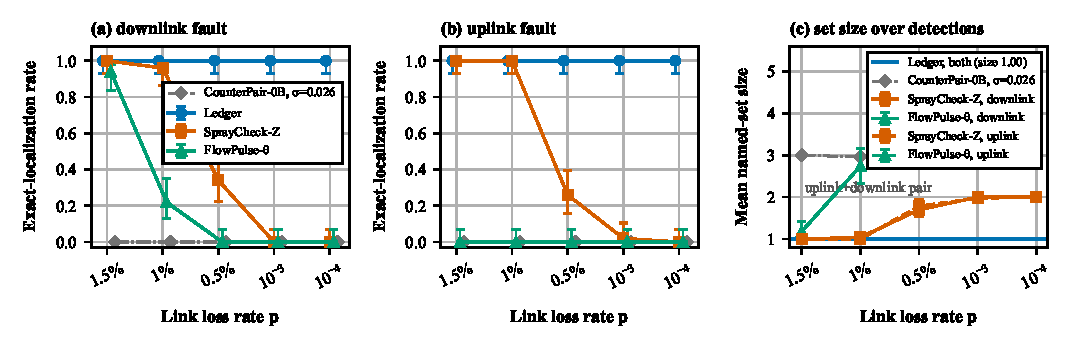
\includegraphics[width=\textwidth]{fig_localization.pdf}
\caption{Localization under spraying, 50 seeds per cell with 95 percent intervals. (a) Exact-localization rate for a downlink fault. (b) Exact-localization rate for an uplink fault. (c) Mean size of the named set over detections: 1 is the exact directed link, 2 is the uplink and downlink pair; the ledger's set size is 1.00 in every cell, and a missing point means the arm detected nothing.}
\label{fig:localization}
\end{figure*}

\textbf{The oracle row, and the counter pair beside it.} In every cell of both families the ledger's exact rate was 1.00 [0.93, 1.00], its mean set size was exactly 1.00, and it named a healthy link in no seed. This is definitional: it detects in every seed with a false-positive rate of 0.00 (Section~\ref{sec:detection}), and the sublink it rejects is a directed link. The counter pair read at one instant reproduced the row exactly. The counter pair read with the measured best-case skew of $\sigma=0.026$ named a set of about three links in every seed and never the faulty link alone. The reason is that the phantom loss of Section~\ref{sec:detection} makes two or three healthy links look faulty beside the real one; the same information, read on two switches, no longer localizes. The measured result of this section is therefore the passive arms' aliasing and the counter pair's skew, with the ledger as the reference.

\textbf{SprayCheck-Z ties at high loss and degrades to the pair at low loss.} At 1.5 percent in both families and at 1.0 percent for the uplink, SprayCheck's cross-leaf intersection resolved the fault to one directed link as well as the ledger did. There were no discordant seeds between the two arms in those cells, and we report the tie as a null result rather than as a test statistic, since a McNemar test with no discordant pairs is uninformative. At 0.5 percent its exact rate fell to 0.34 for the downlink and 0.26 for the uplink. At $10^{-3}$ it fell to 0.00 and 0.02 with a mean set size of 2.00, i.e., the uplink and downlink pair its paper says an uncorroborated report is left with. The reason is that at those rates its Z-test flags the faulty spine on too few distinct leaves to complete the intersection, so it can name the spine but not the directed link. Every such pair contains one healthy link, which is why the ambiguous column reaches 1.00 there: a repair that acted on the set would touch the wrong hop half the time. At $10^{-4}$ it missed in 74 percent of seeds even under the generous budget.

\textbf{FlowPulse-$\theta$ cannot localize an uplink fault at any rate.} For a downlink fault it was exact in 94 percent of seeds at 1.5 percent, fell to 22 percent at 1.0 percent with a mean set size of 2.74, because its all-or-one rule landed in neither branch and returned the port's whole candidate set, and missed at 0.5 percent and below. For an uplink fault it missed in every seed at every rate, including 1.5 percent. The reason is that a single sender's loss moves the aggregate load of the ingress port by only about $1/\!\text{(number of senders)}$ of the drop rate, here about 0.5 percent for a 1.5 percent uplink loss shared by three senders, which never clears the paper's fixed one-percent threshold. This is faithful to FlowPulse's own design: in its native setting one sender occupies each port and an uplink fault is the whole port's load. Under multi-sender spraying the same fault is diluted below its threshold. The gap is a property of the sprayed fabric, reproduced, not a handicap imposed on the baseline.

\textbf{Boundary.} These results hold for one independent fault on a fabric of four leaves and eight spines with uniform spray. FlowPulse's dilution grows with the number of senders per port, so it is worse at larger radix; SprayCheck's intersection improves with more leaves but needs a longer corroborating round. We expect the ordering of the arms to survive both changes, while the exact crossover rates are properties of this fabric, not universal constants.

\section{The Ledger on Silicon (O3)}
\label{sec:silicon}

The replay harness models the ledger's counters. This section measures them. Because the passive detectors are host-side systems that cannot run on our fabric, silicon cannot host the head-to-head; what it can do is show that the ledger's own side of the comparison is measured rather than modelled, at the same loss rates, on a real switch. We expect the ledger to recover the injected loss exactly at every rate, on the first read after the traffic, and to attribute it to the injected directed link alone; a one-packet discrepancy may appear where a loss trails the last survivor of a read.

\begin{table}[t]
\caption{Recovery of injected loss on the Tofino switch, one sublink, exact injector: packets sent $N$, drops armed $D$, register deltas, and the recovered loss $\Delta\mathit{seq}-\Delta\mathit{obs}$. Every cell recovered $D$ exactly, and the two clean cells recovered 0.}
\label{tab:silicon}
\centering
\footnotesize
\begin{tabular}{@{}lrrrrrc@{}}
\toprule
$D/N$ & $N$ & $D$ & $\Delta\mathit{seq}$ & $\Delta\mathit{obs}$ & Recovered & Match \\
\midrule
clean     & 20\,000 & 0  & 20\,000 & 20\,000 & 0  & yes \\
clean     & 20\,000 & 0  & 22\,050 & 22\,050 & 0  & yes \\
$10^{-2}$ & 5\,000  & 50 & 5\,000  & 4\,950  & 50 & yes \\
$10^{-2}$ & 5\,000  & 50 & 5\,000  & 4\,950  & 50 & yes \\
$10^{-3}$ & 30\,000 & 30 & 30\,000 & 29\,970 & 30 & yes \\
$10^{-3}$ & 30\,000 & 30 & 30\,000 & 29\,970 & 30 & yes \\
$5\!\times\!10^{-4}$ & 40\,000 & 20 & 40\,000 & 39\,980 & 20 & yes \\
$10^{-4}$ & 60\,000 & 6  & 60\,000 & 59\,994 & 6  & yes \\
$10^{-4}$ & 60\,000 & 6  & 60\,000 & 59\,994 & 6  & yes \\
\bottomrule
\end{tabular}
\end{table}

\begin{figure*}[t]
\centering
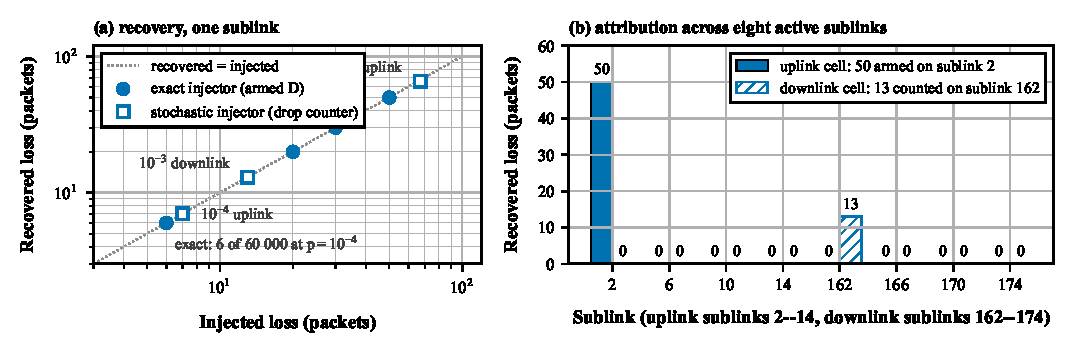
\includegraphics[width=\textwidth]{fig_silicon.pdf}
\caption{The ledger on the Tofino switch. (a) Recovered loss against injected loss on one sublink, on logarithmic axes, for the exact injector, whose ground truth is the armed count, and for the stochastic injector, whose ground truth is its own drop counter; every point lies on the identity except the $10^{-3}$ uplink cell, one packet below it. (b) Recovered loss on each of the eight active sublinks for the uplink cell and for the downlink cell; only the injected sublink recovers a non-zero loss in each.}
\label{fig:silicon}
\end{figure*}

\textbf{Recovery across the loss regime.} Table~\ref{tab:silicon} and Figure~\ref{fig:silicon}(a) present nine cells on one uplink sublink. In every cell the recovered loss equals the armed drop count exactly, from 50 drops in 5\,000 packets down to 6 drops in 60\,000, and the two clean cells, together more than 42\,000 packets, recovered 0. The ledger reported each value on the first census read after the traffic. It does not accumulate packets toward a statistical threshold, because Equation~\eqref{eq:loss} counts the missing packets rather than inferring them. This is the structural contrast with Section~\ref{sec:detection}. At $10^{-4}$, where the passive detectors detect nothing within the budget, the witness recovers the six lost packets on real hardware.

\textbf{Random drops.} A scheduled burst is the easy case, so we repeated the measurement with the stochastic injector, which drops each packet independently with probability $W/2^{16}$, and we compared the recovered loss with the injector's own counter of packets it dropped. At a target of $10^{-4}$ ($W=7$, realized rate $1.07\times10^{-4}$) on 60\,000 packets, the ledger recovered 7 and the injector counted 7. At a target of $10^{-3}$ ($W=66$, realized $1.01\times10^{-3}$) the ledger recovered 66 and the injector counted 67. Two facts in the data account for the one-packet gap, and we believe neither is a recovery error. First, a drop with no later survivor on the sublink is not exposed until the next survivor advances the frontier, which is the trailing-loss property of Section~\ref{sec:ledger}. Second, on that uplink egress the injector's offered count ran about 180 to 190 packets above the 60\,000 host departures. In other words, a small population of packets that are not part of the host-stamped sequence crossed the same egress, and the injector saw them but the ledger did not. The recovered value tracks the loss of stamped packets, which is the quantity the ledger is defined to recover.

\textbf{Localization on the uplink.} Figure~\ref{fig:silicon}(b) shows both attribution cells. We armed 50 drops on one uplink sublink and sent 20\,000 packets across all four traffic classes, 5\,000 each, so that every one of the eight tracked sublinks carried traffic. The injected sublink recovered 50, and the other seven recovered 0. Among the seven is the downlink sublink of the same traffic class, which showed 4\,950 arrivals rather than 5\,000, because the 50 packets dropped on the uplink never reached the downlink to be stamped. It manufactured no loss there, since its $\Delta\mathit{seq}$ and $\Delta\mathit{obs}$ advanced together.

\textbf{Localization on the downlink.} The mirror case is the one the passive vantage cannot resolve. We armed the stochastic injector at $10^{-3}$ on a downlink sublink and sent 80\,000 packets across all four classes, 20\,000 each. The downlink sublink recovered 13 and the injector counted 13. Every other sublink recovered 0, including the uplink sublink of the same class, whose 20\,000 packets had all been witnessed before the downlink drop. On silicon, then, a downlink grayhole is attributed to the downlink directed link alone and an uplink grayhole to the uplink alone, with zero false attribution on seven active sublinks in each case. This is the disaliasing property the replay harness measured in Section~\ref{sec:localization}.

\textbf{Scope.} These cells measure recovery fidelity and false attribution for one independent fault at a time on a 4-leaf, 2-spine virtual fabric. The recovered loss is magnitude-based and is the same for a burst and for dispersed drops of the same count; the one-gap-per-discontinuity property is covered by the model tests of Section~\ref{sec:method}, not here. The added-load figure of Section~\ref{sec:cost} is computed from the header size, not measured as saturating throughput.

\section{The Boundary: Correlated Faults (O4)}
\label{sec:robustness}

Every result so far injects one independent fault. This section asks whether the advantage survives several faults at once, whether it survives a correlated, fleet-wide shift in loss, and whether it survives persistent congestion loss on a subset of links. The last is the shape of incast at a collective's reduction point, and it is more likely in a training fabric than a uniform shift. It is a gate rather than a pass: where the advantage collapses, that bounds the headline claims, and the first two regimes were pre-registered as that boundary. The harness of Section~\ref{sec:method} drives four regimes over the 64 directed links of the two-hop fabric, 50 seeds per cell and 40 post-onset epochs, with the ledger's controller unmodified. Two anchors accompany every cell: a do-nothing arm that never acts, and an oracle that returns the true set. The injected loss was verified in the data of every cell, not in the configuration. Figure~\ref{fig:correlated} summarizes the four regimes; the full per-cell tables, with intervals and both the window and final-epoch scores, are in the artifact.

\begin{figure*}[t]
\centering
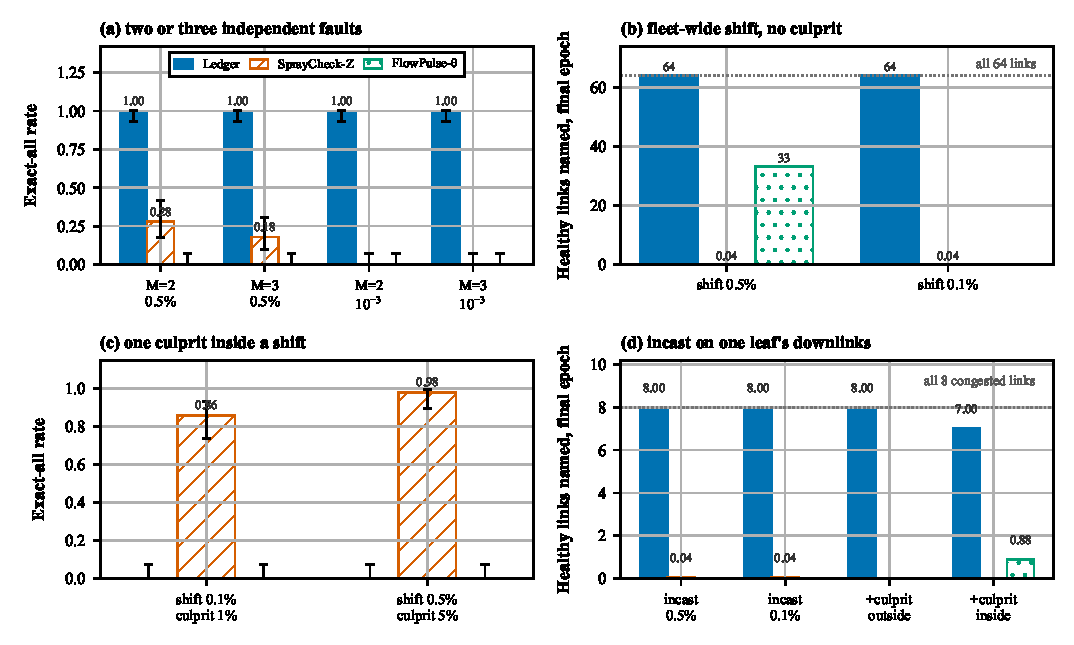
\includegraphics[width=\textwidth]{fig_correlated.pdf}
\caption{The correlated-fault gate, 50 seeds per cell over 40 post-onset epochs on 64 directed links. (a) Exact-all rate, with 95 percent intervals, for two and three simultaneous independent faults. (b) Healthy links falsely named at the final epoch under a fleet-wide shift with no culprit, where the correct answer is zero and 64 is every link. (c) Exact-all rate for one culprit embedded in a shift. (d) Healthy links falsely named at the final epoch when the eight downlinks into one leaf carry persistent congestion loss, alone and with a culprit outside or inside the congested set. The ledger holds in (a) and fails in (b), (c), and (d), where SprayCheck-Z holds.}
\label{fig:correlated}
\end{figure*}

\subsection{Several Independent Faults}

Figure~\ref{fig:correlated}(a) presents the first regime, in which $M\in\{2,3\}$ distinct directed links are faulty at the same rate against a healthy background. The ledger named every one of the faulty links on the first epoch after onset, with no false link, at both 0.5 percent and $10^{-3}$. The reason is that it judges each directed link on that link's own evidence, so a second fault elsewhere in the fabric changes nothing about the first. SprayCheck-Z became worse as faults multiplied. Because several simultaneous failure reports create spurious cross-leaf intersections, it recalled the true faults at 0.5 percent but added 1.2 to 1.4 healthy links per seed. It named exactly the true set in only 18 to 28 percent of seeds. At $10^{-3}$ its recall itself fell to 0.63 to 0.75, and a healthy link was still named at the final epoch in about half the seeds. FlowPulse-$\theta$ missed at these rates, as in the single-fault sweep. The independent-fault advantage therefore appears stronger with several faults than with one, and the spurious-intersection behaviour is a limitation of the passive localizer that we have not found reported elsewhere.

\subsection{A Fleet-Wide Shift With No Culprit}

Figure~\ref{fig:correlated}(b) presents the second regime, in which every directed link's loss rises to the same level and no link is individually at fault, so the correct answer is to name nothing. The ledger failed this gate. It named all 64 directed links in every seed, on every epoch through the end of the window, which is worse than doing nothing. The reason is that its fleet floor is a leave-one-out estimate that lags a shift shared by every link. Each link's ratio then reads the shifted but healthy rate as strong evidence, and e-BH rejects nearly every link. The rejected links leave the pool from which the floor is estimated, and the fleet latches. We had predicted this failure from our own analysis of the decision rule before the gate was run, and the gate reproduced it on fresh seeds. SprayCheck-Z was the arm that held here, with a false-positive rate of 0.02 at the final epoch. Its Z-test normalizes each flow by that flow's own observed count, which falls with the shift, so a uniform shift can cancel. FlowPulse-$\theta$ flagged nearly every port when the shift's two-hop deficit crossed its one-percent threshold and flagged nothing when it did not; below the threshold it is blind rather than resistant.

\subsection{A Culprit Inside the Shift}

Figure~\ref{fig:correlated}(c) presents the third regime, a shift plus one link worse than the shifted background. The ledger did find the culprit, in every seed and on the first epoch, but it drowned the culprit among the other 63 links, so its exact-all rate was 0.00 and its answer was not actionable. SprayCheck-Z isolated the culprit cleanly against the shifted background, with exact-all rates of 0.86 and 0.98 and no healthy link named at the final epoch, for the same reason that let it hold in the second regime. In this regime, then, the exact directed-link localization that is the ledger's advantage under independent faults becomes SprayCheck's advantage.

\subsection{Congestion Loss on a Subset of Links}

Figure~\ref{fig:correlated}(d) presents the fourth regime. The eight downlinks into one leaf carry a persistent elevated loss of 0.5 or 0.1 percent while the other 56 links stay at the floor, first with no fault anywhere and then with a 1 percent culprit on an uplink outside the congested set or on a downlink inside it. This is congestion loss, not a fault, and the correct answer names none of the eight congested links. The ledger named all eight, in every seed, at every epoch, and with a culprit present it found the culprit in every seed but could not separate it from the seven or eight congested links beside it, so its exact-all rate was 0.00. The reason is not the floor this time, which the 56 healthy links keep well estimated; it is that the ledger is a loss counter, and congestion loss is loss. Equation~\eqref{eq:loss} counts the packets a queue dropped exactly as it counts the packets a damaged optic dropped, and nothing in the decision rule asks why. SprayCheck-Z held again, naming a congested link at the final epoch in 2 percent of seeds and isolating the culprit in 92 to 96 percent, because its per-flow normalization cancels a loss that every flow through the congested leaf shares. FlowPulse-$\theta$ was blind to the congestion at both levels, as its per-port deficit stayed below its threshold, and named three links when the culprit sat inside the congested set. We had expected this result from the analysis of Section~\ref{sec:ledger}, and we report it because an operator is likely to meet incast far more often than a uniform fleet-wide shift. Section~\ref{sec:discussion} states what a fix needs: a signal that separates queue loss from link loss, which the testbed's queue-depth metadata can supply and which this paper does not evaluate.

\subsection{What the Gate Decides}

The advantage holds, and widens, for several simultaneous independent faults; it fails under a common-mode shift, and it fails under persistent congestion loss on a subset of links. Consequently, the claims of Sections~\ref{sec:detection} to~\ref{sec:silicon} are stated for one or several independent per-directed-link faults on a fabric whose remaining links lose packets only at the background floor. We state the converse as plainly. Where loss is shared, whether by every link or by the links behind one congested queue, the ledger's absolute test names the shared loss as faults, and a relative passive test is the better tool. Section~\ref{sec:discussion} discusses what a fix would need.

\section{Cost}
\label{sec:cost}

The passive detectors pay nothing on the wire, and the ledger does. This section reports the ledger's cost in the currency each baseline paper uses for its own, from the compiler's resource report on the switch's own software development kit, not from an estimate. Table~\ref{tab:cost} presents it beside the numbers the two baseline papers report for themselves.

\begin{table}[t]
\caption{Cost of the ledger beside the self-reported cost of the passive detectors. Ledger numbers are from the hardware compile on SDE 9.13.2, which matched the 9.13.1 compile exactly; the 4-byte column is the earlier version that also carried a link identifier. SprayCheck's state is under 2 KB in total but covers one flow at a time, rotating about once a minute; FlowPulse's paper states no memory figure. We have not reimplemented either in P4, so no stage count exists for them.}
\label{tab:cost}
\centering
\footnotesize
\begin{tabular}{@{}lccc@{}}
\toprule
 & Ledger, 2 B & Ledger, 4 B & Passive \\
\midrule
Wire bytes per packet & 2 & 4 & 0 \\
Added load (1400 B) & 0.14\% & 0.28\% & 0 \\
State per directed sublink & 6 B & 6 B & see caption \\
Sublinks covered at once & 1024 & 1024 & one flow / port \\
Ingress / egress stages & 12 / 5 & 11 / 5 & -- \\
SRAM / TCAM blocks & 91 / 16 & 89 / 15 & -- \\
\bottomrule
\end{tabular}
\end{table}

\textbf{Wire.} The witness is two bytes per packet, i.e., about 0.14 percent of a 1400-byte payload, computed as $2/1404$. The earlier four-byte version, which also carried a link identifier, cost 0.28 percent, the same order as the $\pm$0.25 percent flow-priority distortion SprayCheck reports for its own prioritized flows~\cite{spraycheck}. The stamp is stripped before host delivery, so the cost is bandwidth on every fabric hop and nothing at the endpoints.

\textbf{State.} Each directed sublink holds a 16-bit sequence register and a 32-bit observed-count register, six bytes, and the program tracks all 1024 sublinks continuously. SprayCheck's own state is under two kilobytes, but it instruments one flow at a time and takes about a minute to rotate to the next~\cite{spraycheck}; FlowPulse's paper does not state a memory figure~\cite{flowpulse}. The trade is continuous per-link coverage of the whole fabric for a fixed per-packet tag, against zero tag for a rotating sample.

\textbf{Pipeline.} Halving the wire cost was not free. Reconstructing the directed link at ingress from the port and the spray field added two narrow tables, and the compiler placed them in a new stage. The program went from 11 to 12 ingress stages, which is the hardware ceiling of the Tofino~1, with 5 egress stages unchanged. It also went from 89 to 91 SRAM blocks and from 15 to 16 TCAM blocks. The compile was byte-for-byte identical on the laptop SDE 9.13.1 and the switch's 9.13.2, with zero errors and the same five warnings on both. The stage cost follows from a choice we made before compiling. To avoid destabilizing logic that other parts of the program rely on, we added narrow tables rather than widen the key of an existing multi-purpose port-role table. Consequently, the program now has no ingress stage headroom, and any future ingress addition must either remove a stage elsewhere or revisit that choice by folding the reconstruction key into the port-role table. We report this as the real cost of the two-byte witness rather than as a footnote, because a reviewer who weights pipeline stages over wire bytes can reasonably prefer the four-byte version.

\section{Discussion and Limitations}
\label{sec:discussion}

\textbf{What the detection buys at the application.} The paper's motivation is that a grayhole at $10^{-3}$ to $10^{-4}$ slows every collective that crosses it, and the reader is owed the measurement that tests it. We ran one, and it is unfavourable to the motivation as first stated. We simulated a mixture-of-experts collective at packet level on a 1024-uplink sprayed fabric, with a $10^{-3}$ grayhole injected on a fully loaded uplink, 255 silent drops over the job, and retransmission-timeout recovery at its worst-case setting of 40 ms. The collective's completion time rose by 1.36 percent over the fault-free run (3.588 s to 3.636 s). Because the timeout was at its largest value, the figure should bound every faster recovery setting. Because the simulator's measurement layer has no mitigation actuator, the fault-free run is the only ceiling on what any mitigation could recover: at most 1.36 percent at this operating point. About 99.5 percent of the drops appear to have been absorbed by the collective's pipelining, since a timeout on one chunk overlaps other chunks' slack and only the worst straggler moves the barrier. Consequently, the value of naming a $10^{-3}$ link is not the completion time of the collective that is running when it is named. It lies elsewhere, and we state where without claiming more than the measurement supports. First, a link losing at $10^{-3}$ from a physical cause is a link that is degrading toward $10^{-2}$ or toward a blackhole; Section~\ref{sec:background} already assumes, with CorrOpt~\cite{corropt}, that such causes persist until repaired, so early naming has repair and attribution value that a single completion-time measurement cannot capture. Second, the 1.36 percent is on one collective, and a fleet runs thousands of links continuously, so the aggregate is not 1.36 percent of one job. Last, the contribution of this paper is the measurement instrument and its boundary. The application-level value of low-loss detection is an open question, and our own simulation bounds it at about 1.4 percent per collective under timeout-dominated recovery.

\textbf{Common-mode and congestion loss.} The failures of Section~\ref{sec:robustness} are the ledger's largest limitation, and they are properties of the decision rule, not of the witness. The registers still recover each link's loss exactly under a fleet-wide shift and under incast. What fails is a comparison against a floor that moves with the fault in the first case, and the absence of any question about the cause of the loss in the second. A fix for the first may need a guard that detects when the floor itself is drifting, or a corroboration gate that requires a link's ratio to stand out relative to its neighbours as well as relative to the floor, i.e., the relative normalization that lets SprayCheck hold in that regime. A fix for the second needs a signal that separates queue loss from link loss; the testbed exposes per-packet queue depth in the egress pipeline, so a stamp that carries it, or a gate that consults it, is the obvious candidate. Both are design work with their own evaluation, and this paper does not do them.

\textbf{What the two bytes buy, and what they do not.} Equation~\eqref{eq:loss} contains no information a zero-byte counter pair lacks, and Section~\ref{sec:detection} shows the two are identical when the pair is read at one instant. What the stamp buys is that the sender's count arrives in band, so the receiver holds both terms of the difference and reads them in one operation. The pair's tolerance to read timing is about ten microseconds across two switches, against a measured 2.6 ms for the nearest pairwise read and 350 ms for a census on our controller. The stamp does not buy a better inference: the localization score of 1.00 in Section~\ref{sec:localization} is definitional given per-directed-link counts, and we present the ledger there as the oracle row against which the passive detectors' aliasing is measured, not as a result.

\textbf{A synchronized counter snapshot.} The read-skew argument invites an obvious reply: do not read the two registers at one instant, latch them at one instant and read them at leisure. If both switches copied their per-directed-link counters into shadow registers on a common epoch boundary derived from precision time, the controller could take its full 350 ms to collect them. The skew term would then be sub-microsecond, an order below the tolerance Section~\ref{sec:detection} establishes, and the counter pair would match the witness at zero wire bytes. This is the alternate-marking family of loss measurement~\cite{rfc9341}, and RFC 6374 is built around it. We believe the reply holds in principle, and we scope the paper against it. Three things bound it in practice. First, the snapshot is not free in the data plane, and our own history prices it. The program this ledger replaced kept alternating counter banks per epoch with a guard interval. The compile gate that retired it measured the banked scheme at two more tables, three more SRAM blocks, one more stateful ALU, and two more header containers than the ledger at the same stage count, before any time synchronization. It also carried the bank parity in a fabric header byte, so it was not zero-byte either, and a transit stage that failed to preserve that byte produced a 56 percent false-blackhole rate until it was found. A snapshot that keys on time rather than on a carried bit avoids the byte but not the banks. Second, the witness needs no fabric-wide coordination: no time distribution, no trusted common time base, and no agreement between two switches about when an epoch began. That is the operational asymmetry that survives the reply. Third, and stated plainly, an operator who has precision time on every switch and can afford the second register bank and the bank swap should prefer the synchronized counter pair, and the witness is then unnecessary. We did not build the synchronized variant; its stage cost on this program is an estimate from the banked scheme we did build.

\textbf{The wire reduction, reconsidered.} Halving the header from four bytes to two cost the program's last ingress stage (Section~\ref{sec:cost}), and the soak below shows it also introduced an anomaly the four-byte program did not have and a structural aliasing of traffic that carries no real spray choice. Neither header escapes the 16-bit wrap bound, since both carry a 16-bit sequence. An operator who weights pipeline headroom or the open anomaly over one byte per packet per hop can reasonably prefer the four-byte program, and the evidence in this paper now points that way rather than merely permitting it. We report both because the trade should be made rather than assumed.

\textbf{The anomaly on unmeasured sublinks, as far as the evidence goes.} During a 57-cycle soak of the two-byte program, the injected-loss recovery passed in every cycle. However, two sublinks that were neither armed nor measured each showed one stamped packet with no matching arrival during clean traffic, a signature not seen across about 3\,200 historical cycles of the four-byte program. We took the investigation as far as the shared hardware allowed. Physical-layer loss was ruled out by port-level media-access counters (9\,224 frames sent and received) and ambient noise by a fully idle window that moved no register. A byte-identical build of the four-byte source, deployed through the same pipeline and run with the same script immediately afterward, showed 0 anomalies in 100 cycles against 2 in 57 for the two-byte build, which isolates the anomaly to the wire-reduction build rather than the testbed. A probe with no injector table writes reproduced it, which rules out the control-plane writes that accompanied the first two occurrences. An idle-then-burst trigger looked confirmed at 3 of 5 post-idle bursts, then two further runs with the corrected instrument found 0 of 9. The honest count is therefore 3 of 14, and the surviving hypothesis is a genuinely cold fabric after a fresh program load rather than mid-session idleness. The root cause is not established, and the fresh-load protocol that would settle it needs its own bring-up budget. Every number in this paper comes from armed, measured sublinks with baseline and post-traffic reads, and none is affected. However, a claim of zero false positives must be read beside a one-packet phantom loss that recurs on the same program, at a rate near 2 per 57 cycles, on unmeasured sublinks.

\textbf{A structural aliasing introduced by the wire reduction.} While restoring the two-byte program after the comparison above, a census of traffic classes outside the probe's set showed phantom arrivals with no stamps on two classes, reproduced across two independent bring-ups. The explanation is mechanistic. Bring-up's own port-verification frames carry no real spray choice and arrive with a spray field of zero, and the new ingress reconstruction maps every frame with spray zero to the first virtual link regardless of which leaf sent it, where the old design read the link identifier the sending egress had written. On the testbed this never touched a measured sublink. In a production fabric, control and management traffic that is stamped but not sprayed would be attributed to one link's counters, and the two-byte design needs either a table entry that excludes unsprayed traffic from the stamp or a spray value reserved for it. We record this as a correctness cost of the reduction that Section~\ref{sec:cost} did not price.

\textbf{Silicon scope.} Section~\ref{sec:silicon} states the limits of the silicon cells: a virtual fabric, one percent of a port, one sublink, computed rather than measured added load, and a one-packet discrepancy explained but not re-measured. The stage budget is that of a stripped program, forwarding plus the ledger. A production leaf program that also carries load balancing, transport offload, access control, tunnelling, and quality of service does not have a spare stage on a Tofino~1, and whether the ledger fits beside such a program, or on a Tofino~2, is not measured here.

\textbf{Generality.} The replay fabric has four leaves and eight spines with uniform spray. FlowPulse's dilution grows with senders per port and SprayCheck's intersection improves with leaves, so we expect the ordering of the arms to survive a change of radix while the crossover rates are properties of this fabric. The $1/p^2$ form of Proposition~\ref{prop:cost} does not depend on the topology; its constants do, through the floor and the epoch volume, and Section~\ref{sec:detection} sweeps both.

\section{Related Work}
\label{sec:related}

Table~\ref{tab:related} positions the ledger against the systems closest to it on the axes this paper measures. We group them into four families.

\begin{table*}[t]
\caption{Prior systems on the axes this paper measures. DL: directed link. ``Not addressed'' means the paper does not target that axis. The ledger row restates measurements from Sections~\ref{sec:detection} to~\ref{sec:cost}; every other cell is taken from the cited paper.}
\label{tab:related}
\centering
\scriptsize
\setlength{\tabcolsep}{2pt}
\begin{tabular}{@{}>{\raggedright\arraybackslash}p{1.55cm}>{\raggedright\arraybackslash}p{2.55cm}>{\raggedright\arraybackslash}p{1.7cm}>{\raggedright\arraybackslash}p{1.35cm}>{\raggedright\arraybackslash}p{1.8cm}>{\raggedright\arraybackslash}p{2.95cm}>{\raggedright\arraybackslash}p{2.75cm}>{\raggedright\arraybackslash}p{1.95cm}@{}}
\toprule
System & Primitive & Vantage & Per-DL & Under spraying & Low-loss detection cost & Localization under spraying & Restoration \\
\midrule
NetSeer~\cite{netseer} & 4 B egress per-DL sequence & in-fabric, passive & exact DL & not addressed & next packet, $\Theta(1)$; not measured under spray & exact DL, not spray-measured & no \\
LinkGuardian~\cite{linkguardian} & 3 B sequence, era bit, dummy packet & in-fabric, passive & exact DL & not addressed & $\Theta(1)$ & exact DL, not spray-measured & link-local retransmit \\
LossRadar~\cite{lossradar} & invertible Bloom filters at both ends & in-fabric, passive digest & exact DL & not addressed & per-packet decode only below about 0.1\% & exact DL below 0.1\%; counts above & no \\
UEC LLR~\cite{uec} & per-link sequence in the MAC & in-fabric, passive & exact DL & in MAC, not measured & retry, $\Theta(1)$ & exact DL, no spray number & link-layer retry \\
RFC 6374~\cite{rfc6374} & TX/RX counter pairs & in-fabric, passive & if measured per DL & attribution fails & epoch-skew limited & none under spray & no \\
SprayCheck~\cite{spraycheck} & per-(leaf, spine) RX Z-test, cross-leaf intersection & in-fabric counts, passive & by intersection & yes & 0.78 at $10^{-3}$, 0.00 at $10^{-4}$; about $\Theta(1/p)$ (measured here) & exact DL at 1--1.5\%; pair at $\le 10^{-3}$ (measured here) & no \\
FlowPulse~\cite{flowpulse} & learned per-port load, 1\% threshold & in-fabric + model, passive & per-port rule & uplink diluted by senders & fails at $\le 10^{-3}$ (measured here) & port set or miss; misses uplinks (measured here) & no \\
dShark~\cite{dshark} & mirrored per-hop trace analysis & host, post hoc & hop via TTL & not a spray study & localizes blackholes; capture drops & hop from trace & no \\
NetBouncer~\cite{netbouncer} & active probes, scalar per link & host, active & per-link scalar & path pinning breaks & link is one resource & per link, no DL under spray & no \\
Bartolini et al.~\cite{bartolini} & identifiability bound & theory & bound & owns the framing & bound, no cost curve & monitor placement & no \\
OmniPath Ping~\cite{omnipath} & in-network per-hop cache, probes & in-fabric, active & per hop & yes (concurrent) & tracing, not a cost study & per hop & no \\
CorrOpt~\cite{corropt} & corruption rate, disable, repair & host + counters & per-link scalar & fixed routing & not a spray localizer & no & disable both directions, repair, re-enable \\
Aegis~\cite{aegis} & enhanced probe sizes & host, active & path & cannot reach spray-hidden links & 64 B probes missed a $>$1 KB fault & path level & quarantine, audit, certify \\
REPS~\cite{reps} & spray load balancer, reroute away & in-fabric balancer & not a localizer & yes, avoidance & no loss localization & no & reroute away, re-explore \\
\midrule
This paper & 2 B egress per-DL sequence, two registers & in-fabric, passive on stamped stream & exact DL & yes & 1.00 at $10^{-3}$ and $10^{-4}$, flat 22 M packets & exact DL, set size 1, both families & not claimed \\
\bottomrule
\end{tabular}
\end{table*}

\textbf{In-fabric loss witnesses.} NetSeer~\cite{netseer} inserts a per-neighbour sequence number at egress and treats an inconsecutive number at the downstream ingress as a drop, which is exactly the ledger's encoding at four bytes. LinkGuardian~\cite{linkguardian} adds an era bit and a dummy packet and retransmits the lost packet across the link. LossRadar~\cite{lossradar} stores packet digests in invertible Bloom filters at both ends of a link and decodes the difference, which its authors state works per packet only below about 0.1 percent loss. The Ultra Ethernet link-layer retry~\cite{uec} places the sequence in the MAC, and RFC 6374~\cite{rfc6374} pairs transmit and receive counters per measurement entity. These systems own the primitive this paper uses, and we claim none of it. The counter pair of RFC 6374 is, in the information it holds, the same as the witness; Section~\ref{sec:detection} measures the read skew that separates them, which Table~\ref{tab:related} calls skew-limited and which no prior system quantifies. Compared to this work, none of them reports what the witness buys or costs on a sprayed fabric at $10^{-3}$ to $10^{-4}$, measured against the passive detectors built for that fabric.

\textbf{Passive detectors for sprayed fabrics.} SprayCheck~\cite{spraycheck} and FlowPulse~\cite{flowpulse} are the direct comparators of this paper and the state of the art for sprayed fabrics. Both are zero-byte, both are deployable on existing counters, and SprayCheck reports zero added network load. The ledger does not dominate them on added load, because it pays two bytes per packet and they pay nothing. What it buys, measured in Sections~\ref{sec:detection} and~\ref{sec:localization}, is a detection cost that does not grow as $1/p$ and a localization that does not alias the uplink and downlink pair, and both follow from holding each directed link's own transmit count. Under a common-mode shift, SprayCheck's relative test can hold where the ledger's absolute one cannot (Section~\ref{sec:robustness}). OmniPath Ping~\cite{omnipath} is concurrent work that addresses path ambiguity under spraying with an in-network per-hop cache and active probes; it is a tracing tool rather than a cost study, and it owns the problem statement of active measurement under spraying.

\textbf{Active probing and tomography.} dShark~\cite{dshark} localizes drops, including silent ones, by analysing mirrored per-hop traces on hosts after the fact, at a cost of mirroring the traffic and of capture drops that can hide real drops. The ledger's only edge over it is that two registers per sublink on a rerouteable resource are cheaper and act in place, not that it can find anything dShark cannot. NetBouncer~\cite{netbouncer}, 007~\cite{007}, deTector~\cite{detector}, Pingmesh~\cite{pingmesh}, and Everflow~\cite{everflow} probe or trace paths from hosts and infer per-link health; under per-packet spraying a probe cannot pin its path, so these systems localize to a path or a scalar per link rather than to a directed link. Bartolini et al.~\cite{bartolini} give the identifiability bounds of Boolean tomography as a function of routing, which is the framing in which the aliasing limit of Section~\ref{sec:limits} sits; the ledger sidesteps the bound by adding information rather than by a better inference, and we make no identifiability claim.

\textbf{Repair and restoration.} CorrOpt~\cite{corropt} disables a corrupting link in both directions and re-enables it after repair; Aegis~\cite{aegis} quarantines, audits with host-generated traffic, and certifies; REPS~\cite{reps} reroutes sprayed traffic away from a lossy path and re-explores it. All three re-admit on evidence from real or generated traffic, which a link that spraying has starved cannot supply. Compared to this work, they serve a different objective, the lifecycle after localization, and we cite them to bound what the measurement enables rather than to claim restoration. We have found no prior system that reports the head-to-head of Table~\ref{tab:related}'s last row against its SprayCheck and FlowPulse rows on a sprayed fabric, on silicon, at the low-loss regime, and that row is what this paper adds.

\section{Conclusion}
\label{sec:conclusion}

We measured what a two-byte per-directed-link witness buys, and costs, on a packet-sprayed fabric against the two most recent passive detectors built for such fabrics and against a zero-byte counter pair with identical information, all replayed over one shared stream, and we measured the witness itself on an Intel Tofino switch. A count test and the witness both pay packets that grow as the inverse square of the loss rate, and the witness divides the constant by the background floor. From 1.5 percent loss down to $10^{-4}$ it detects on one epoch of 2 million packets, where the passive cost reaches 94 million at $10^{-3}$ and exceeds a 160-million-packet budget at $10^{-4}$; its own wall sits at a few times the floor and moves with it. It names the exact directed link where the passive detectors return the uplink and downlink pair. A counter pair matches it only when both registers are read within about ten microseconds, four orders of magnitude tighter than the census we measured, so what the two bytes buy is in-band alignment rather than information. On silicon the ledger recovers injected loss exactly down to six packets in sixty thousand. It costs 0.14 to 2.4 percent of the wire depending on packet size, one pipeline stage, a rate bound set by the 16-bit sequence and the read loop, and two defects the reduction to two bytes introduced. The advantage widens with several independent faults and fails under a fleet-wide shift and under incast, where a relative passive test is the better tool, so every claim is stated for independent faults on a fabric that otherwise loses at its floor. Our own simulation bounds the completion-time value of naming a $10^{-3}$ link at 1.4 percent per collective. The witness is an existing primitive; the contribution is the measurement, its cost, and its boundary. In future work, we intend to design and evaluate a gate that separates shared loss, whether fleet-wide or behind one congested queue, from link loss, so that the ledger's exact localization survives it.


\section*{Acknowledgment}
[Funding and testbed acknowledgments to be added by the author.]

\bibliographystyle{IEEEtran}
\bibliography{references}

\begin{IEEEbiographynophoto}{Philip Akekulip}
[Biography to be added by the author.]
\end{IEEEbiographynophoto}

\end{document}
